\documentclass[12pt, a4, twoside]{article}
\usepackage[utf8]{inputenc}
\usepackage{graphicx}
\usepackage{algorithm}
\usepackage{algpseudocode}
\usepackage{multido}
\usepackage{amsmath}
\usepackage{amsfonts}
\usepackage{hyperref}
\usepackage{mathtools}
\usepackage{tikz}
\usepackage{booktabs}
\DeclarePairedDelimiter\ceil{\lceil}{\rceil}
\DeclarePairedDelimiter\floor{\lfloor}{\rfloor}

\hypersetup{
    colorlinks=true,
    linkcolor=blue,
    filecolor=magenta,
    urlcolor=cyan,
}
\algnewcommand{\parState}[1]{\State\textbf{in parallel do} #1}

\usepackage[backend=bibtex]{biblatex}
\addbibresource{m2l.bib}

\title{Accelerating the Multipole to Local Field Translations}
\author{Srinath Kailasa \thanks{srinath.kailasa.18@ucl.ac.uk} \\ \small University College London}

\date{\today}

\begin{document}

\maketitle

\tableofcontents

\section{Introduction}

The fast multipole method (FMM) was originally motivated by $N$-body problems, such as those found in electrostatics and gravitation. This $O(N^2)$ problem is analogous to a matrix vector product (matvec). The FMM accelerates the computation of this matvec to just $O(N)$ or $O(N \log N)$ depending on the underlying kernel function. The former is typically achieved when the problem is such that a subset of particles can be thought to interact only with a constant number of other particles, or groups, and is the case for the kernels we study, which can be considered to be asymptotically smooth. e.g.

\begin{flalign}
    \frac{1}{(r^2 + c^2)^{\frac{n}{2}}}
    \label{eq:asymptotically_smooth_kernel}
\end{flalign}

where $r = \| x-y \|$, $c$ is a given parameter and $n \in \mathbb{N}$. The main idea of the FMM is to separate the near ($\|x-y\| \rightarrow 0$) and far-field ($\|x-y\| \rightarrow \infty$) components of a field actions of a set of particles (e.g. the electric/gravitational potential generated by static charges/masses). The near-field is computed directly, and the far-field is approximated using a divide and conquer strategy by recursion over a hierarchical tree that partitions the region of interest. The algorithm is explained in the literature, and we won't recount it here \cite{Greengard1987}. The algorithmic step of concern is the so-called `M2L' operator, which acts as an approximation of a far-field at a given tree node. This is the most computationally intensive portion of the FMM algorithm, as it needs to be applied to all nodes in a hierarchical tree up to 189 times (in the 3D algorithm). 

The computational optimisation of this operation is the focus of this note. Our choice of kernel functions is deliberate as they are compatible with so-called `black box' FMM methods \cite{Fong2009,Ying2004}. These methods emerged two decades ago, and remain the basis for the highest performance FMM operators as of today \cite{Malhotra2015,wang2021exafmm}, performance in the FMM community is measured in terms of throughput (i.e. particles processed per second). The major benefit of these methods is that unlike the original `analytical' formulations of the FMM, which rely on hand derived representations of multipole/local expansions for each kernel function, they rely \textit{only} on kernel evaluations and are thus highly suitable for generic software implementations that can be specialised to work with a wide variety of kernels.

In this note I summarise different approaches to calculate the M2L operator for black box FMM methods, and various computational \& mathematical optimisations that can be taken to accelerate its calculation. Our group is developing a new distributed \hyperlink{https://github.com/bempp/bempp-rs/tree/main}{FMM software} in Rust as a part of a wider project to develop massively scalable integral equation software. We base our work on the KiFMM introduced by Ying et. al in \cite{Ying2004}, which relies on the method of fundamental solutions (MFS) to approximate the potentials generated by a set of particles, building on the work in \cite{Kailasa2022}.

In this note I summarise the main differences between black box FMMs, and common algorithmic approaches to calculate the M2L. We proceed to discuss a composite approach to approximating the M2L operation, building on previous work in \cite{Malhotra2015,Messner2012}, which we believe will achieve a new benchmark performance for this operation. 

\dots [TODO change eventually when I can take benchmarks!]

We also include an appendix on mathematical details, for example the FFT and SVD algorithms, which are used in approximations.

\subsection{FMM Operator Basics}

In 2D the single-layer Laplacian Green's function is,

\begin{equation}
    G(\mathbf{x}, \mathbf{y}) = -\frac{1}{2\pi} \log \rho
\end{equation}

where $\mathbf{r} = \mathbf{x} - \mathbf{y}$ and $\rho = |\mathbf{r}|$. It is useful to reformulate this using complex numbers, where $G(\mathbf{x}, \mathbf{y}) = \text{Re}\{ \log(z_x - z_y) \}$ where $z_x$ and $z_y$ are complex numbers corresponding to source and target points on the plane. The key idea of the FMM is to encode the potentials fo a set of source densities using a multipole expansion, and a local expansion at places far away from these sources.

Suppose that source densities are supported on a disk centered at $z_c$ with radius $r$. Then for all $z$ outside the disk with radius $R$, ($R>r$) we can represent the potential at $z$ from the source densities using a set of coefficients $\{ a_k, 0 \leq k \leq p \}$ as,

\begin{flalign}
    q(z) = a_0 \log(z-z_c) + \sum_{k=1}^p \frac{a_k}{(z-z_c)^k} + \mathcal{O}\left( \frac{r^p}{R_p} \right), \> \> \text{Multipole Expansion}
\end{flalign}

On the other hand, if the source densities are outside the disk with radius $R$, the potential at a point $z$ inside the disk with radius $r$ can be represented by another set of coefficients $\{ c_l, 0 \leq k \leq p \}$ as,

\begin{flalign}
    q(z) = \sum_{k=0}^p c_k(z-z_c)^k + \mathcal{O}\left(\frac{r^p}{R_p}\right), \> \> \text{Local Expansion}
\end{flalign}

The M2L translation transforms a multipole expansion of a box to a local expansion of another non-adjacent box. Instead of Laurent series, in 3D the far-field is represented using spherical-harmonics.

N.B KIFMM \cite{Ying2004} relies on smoothness of kernel, as well as uniqueness of properly posed interior/exterior Dirichlet problem.

How do you prove that black box methods offer good approximations ? Something that I need to ask about and write down at some point.

The formulation of the operator depends on the algorithm taken \cite{Ying2004,Fong2009}, however in general we will get some kind of matvec, where a translation matrix is applied to a vector of multipole expansion coefficients.

\subsection{Transfer Vectors}

In order to uniquely label M2L interactions we introduce transfer vectors $t = (t_1, t_2, t_3)$, $t \in \mathbb{Z}^3$. They describe the relative positioning of two nodes, $X$ and $Y$, in a hierarchical tree and computed from their centres $t = \frac{c_x - c_y}{w}$ where $w$ is the node width.

\subsection{Interaction Lists}

This section is based on a similar discussion in \cite{Messner2012}, we adapt it here adding expository notes and calculations. A common feature of kernels used in the FMM is translational invariance,

\begin{flalign}\label{eq:translation_invariance_kernel}
    K(x, y) = K(x + v, y+v)
\end{flalign}

where $v \in \mathbb{R}^3$. This alongside with the regular arrangement of interpolation points used in the MFS based KiFMM as well as the Chebyshev based bbFMM mean that it's sufficient to identify unique transfer vectors at each level of the octree, and compute their respective M2L operators. A set of such unique transfer vectors is referred to as an interaction list $T \subset \mathbb{Z}^3$.

If we additionally consinder \textit{asymptotically smooth kernel functions} the near field is limited to transfer vectors satisfying $\|t\| \leq \sqrt{3}$, this leads to $3^3 = 27$ near field interactions in $\mathbb{R}^3$. In a multi-level scheme, these 27 near field interactions contain all $6^3=216$ near and far field interactions of its 8 child nodes. This comes from the fact that far-field interactions for such kernels are defined as nodes that are children of the source node's parent node, which do not neighbour the source node. These far field interactions must also satisfy $\|t \| > \sqrt{3}$, leading to a maximum of $6^3 - 3^3 = 189$ far-field interactions per node. The union of all possible far field interactions for the eight child cells gives $7^3 - 3^3 = 316$ possible interactions. This comes from the fact some subset of translation vectors are non-overlapping for each child, resulting in a total of $7^3$ total interactions for all children, subtracting the near-field interactions which are the same for all children gives the result. Thus 316 is the maximum number of interactions is largest number of different M2L operators that must be computed at each level of the tree in $\mathbb{R}^3$.

If an asymptotically smooth kernel also happens to be homogenous to degree $n$,

\begin{flalign}
    \label{eq:homogenous_kernel}
    K(\alpha r) = \alpha^n K(r)
\end{flalign}

i.e. we can scale the distance between source and target node by a factor of $\alpha$, the potential is scaled by a factor of $\alpha^n$, where $n$ is a kernel function dependent constant, the M2L operators can then be precomputed for a single level and scaled.

\begin{table}[ht]
    \centering
    \begin{tabular}{l|ll}
    \hline
    \textbf{type of kernel function} & \textbf{cells in near field} & \textbf{cells in far field} \\ \hline
    smooth & $\leq$ 27 per leaf &  $\leq$ 316 per level \\ 
    smooth and homog. & $\leq$ 27 per leaf & $\leq$ 316 in total \\ 
    \end{tabular}
    \caption{Number of near and far field interactions by kernel function type}
    \end{table}
    

\subsection{bbFMM}

The basic idea is in this (and other interpolation based FMMs) is as follows. Letting $w_l(x)$ denote interpolating functions,

\begin{flalign}
    K(x, y) \approx \sum_l \sum_m K(x_l, y_m) w_l(x)w_m(y)
\end{flalign}

ie. finding a low-rank approximation of the kernel. The advantage of such methods is that we only require the ability to evaluate the kernel at various points, no kernel dependent analytical expansion is required. The drawback is that the number of terms can be relatively large for a given error tolerance (verify ?).

In Fong et al's approach, a Chebyshev interpolation scheme is used to approximate the far-field behaviour of the kernel. The M2L operator then consists of evaluating the field due to particles located at Chebyshev nodes, this can be effectively compressed using the SVD. If the kernel is translation invariant i.e. of the form $K(x-y)$, the cose of the SVD precomputations reduces to $O(\log N)$ instead of $O(N)$ as we only have to precompute for each level, reduces further if kernel can be scaled between levels.

\subsection{KIFMM}

The KIFMM uses the method of fundamental solutions (MFS) to approximate the field due to a set of discrete charges, an overview of which is given in the appendix. It slightly differs to the bbFMM in formulation, namely through the use of fictitious surfaces, however the fundamental computation remains the same - a matvec.

\subsection{Summary}

Both formulations essentially result in the same kind of computation being taken, some kind of matrix vector product which descrives a convolution operation. There are a couple of approaches that have been taken to accelerate this calculation, we provide an overview of each of these in the following sections, before concluding with a discussion on how we choose to implement the M2L for our software, in light of hardware and software optimisations taken in previous attempts.

\section{Accelerating the M2L with the SVD}

This is the method first presented in \cite{Fong2009}. Consider the application of the M2L operator $K$ to a multipole expansion $w$ to get the check potential $g$.

\begin{equation}
    g = K w
\end{equation}

This can be approximated with a rank $k$ SVD,

\begin{equation}
    \tilde{g} = U_k \Sigma_k V_k^T
\end{equation}


Stacking the M2L operators for all the source nodes in a given target node's interaction list can be done in two ways, column wise,

\begin{flalign}
    K_{\text{fat}} &= \left [ K^1, ..., K^316 \right ] \\
    &= U \Sigma \left [ V^{(1)T}, ..., V^{(316)T} \right ]
\end{flalign}

where we use the fact that there are at most 316 unique orientations for the M2L operator in 3D. Similarly they can be stacked row wise,

\begin{flalign}
    K_{\text{thin}} &= \left [ K^1; ...; K^{316} \right ] \\
    &= \left [ R^{(1)T}; ...; R^{(316)T} \right ]  \Lambda S^T
\end{flalign}

we note that
\begin{flalign}
    K_{\text{thin}}  = K_{\text{fat}}^T 
\end{flalign}

for symmetric kernels.

We can do some algebra to reduce the application cost of $K$ when we've done these two SVDs. Consider the application of a single M2L operator corresponding to a single source box in a target box's interaction list,

\begin{flalign}
    K^{(i)}w = R^{(i)}\Lambda S^T w
\end{flalign}

Using the fact that $S$ is unitary, $S^TS = I$, we can insert into the above equation,

\begin{flalign}
    K^{(i)}w &= R^{(i)}\Lambda S S^T S^T w \\
    &= K^{(i)} SS^T w \\ 
    &= U \Sigma V^{(i)T} SS^T w \\
\end{flalign}

Now using the fact that $U$ is also unitary, such that $U^T U = I$, we find

\begin{flalign}
    K^{(i)}w &= UU^T U \Sigma V^{(i)T} SS^T w \\
    &= U [U^T U \Sigma V^{(i)T} S] S^T w \\
    &= U[U^T K^{(i)} S] S^T w 
\end{flalign}

The term in the brackets can be calculated using the low rank (k-rank) terms from the SVD,

\begin{flalign}
    [U^T K^{(i)} S] &= \Sigma V^{(i)T}S\\
    &= U^T R^{(i)} \Lambda 
\end{flalign}

We call this previous equation the compressed M2L operator,

\begin{flalign}
    C^{i,k} =  U^T K^{(i)} S
\end{flalign}

This object can be pre-computed for each unique interaction. The M2L operation can be then broken down into 4 steps

1. Find the `compressed multipole expansion'

\begin{flalign}
    w_c = S^T w    
\end{flalign}

2. Compute the convolution to find the compressed check potential

\begin{flalign}
    g_c = \sum_{i \in I} C^{i, k} w_c
\end{flalign}

where the sum is over the interaction list $I$.

3. A post processing step to recover the check potential

\begin{flalign}
    g = U g_c
\end{flalign}

4. The calculatation of the local expansion, as usual, in the KIFMM.

Doing this the convolution step is reduced to matrix vector products involving the compressed M2L matrix, which is only of size $k \times k$, rather than $6(p-1)^2 + 2$ where $p$ is the expansion order.

\subsection{Taking Advantage of Modern Compute Architectures}

The Basic Linear Algbebra Suprograms (BLAS) is a specification for a collection of low-level routines for common linear algebra operations, such as scalar and vector addition/multiplication, dot products, and matrix multiplication among other things. The specification is divided into three levels. BLAS2 is concerned with matrix-vector operations, and is usually a memory bound operation as the amount of data movement is significant in comparison to the size of the computation. BLAS3 on the other hand, which is concerned with matrix-matrix operations, is susually compute bound with similar reasoning for why so.

As modern CPUs have a hierarchical memory structure with multiple levels of cache accessing cached data is much faster than accessing main-memory. BLAS3 uses block-partitioning to maximally use cache.

For operations with the same number of FLOPS a BLAS3 operation will be more performant than a BLAS2 one for a given hardware. This is because BLAS3 operations have a higher ratio of computation to memory access. In BLAS3 once a chunk of data is loaded into cache it can be re-used multiple times before being written to main memory, on the other hand in a BLAS2 operation each element of the matrix is used only once resulting in cache-misses. It's therefore preferable to take advantage of this when designing M2L software. Instead of computing the matrix-vector products, we can block together all the right-hand sides sharing an M2L operation at a given tree level and compute a single BLAS3 operation.

In \cite{Messner2012} they describe redundancies in the number M2L operations can be removed as many of them are simple combinations of translations/rotations of a subset of operators when FMM interpolation points arranged on regular grids as is the case in both the bbFMM and the KiFMM. Indeed the 316 unique operators, reduces to just 16 when translations and rotations are taken into account. Despite this, batching by this reduced set of translation operators has little effect on BLAS3 performance on modern CPUs as demonstrated by the experiment below ....

[BLAS3 experiment]



\section{Accelerating M2L with FFT}

The M2L operation can also be accelerated with a fast fourier transform (FFT). The M2L accelerated this way is quite natural, as it's simply a convolution operation, however computing it in practice can be be tricky. Here I document how I've managed to compute it, as well as a summary of the relevant FFT theory as a background.

\subsection{The M2L Translation as a Fourier Convolution}

For the M2L operation we're computing the following convolution,

\begin{flalign}
    \phi(x) = \int G(x-y) q(y)dy
\end{flalign}

where we're attempting to compute the far-field potential as a convolution of the Green's function with a charge distribution (multipole expansion) at some local box. This is definitely somewhere we can apply the FT/FFT. How is this actually done in practice though, we're only concerned about the BBFMM \cite{Fong2009} case where the charge distributions/multipole expansions are placed at regular intervals on the surface of a box enclosing a node in the octree. In the literature there is a significant gap in describing how to actually setup the convolution operation such that we can apply the FFT to accelerate it, I illustrate it pictorially below.

Consider two boxes (source and target) in 2D for simplicity, the expansion order is set to $p=2$

\begin{center}    
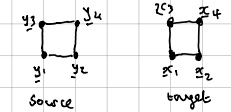
\includegraphics{setup.jpg}
\end{center}

The boxes are referred to as lying in a `surface grid', with the equivalent charges, $q_1,...,q_4$,  placed at $y_1,...y_4$. We embed the unique kernel interactions between these two boxes on a so called `convolution grid', we define them wrt to a fixed point - we can take this to be just $x_1$. These can be pre-computed and stored.

\begin{center}    
    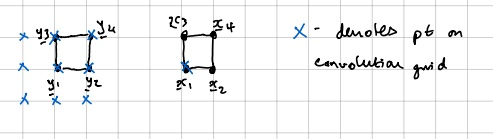
\includegraphics{conv_grid.jpg}
\end{center}

The unique interactions define the convolution grid points. We label these $K_1,...,K_9$. This is how the convolution is defined practically.

\begin{center}    
    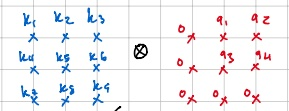
\includegraphics{conv.jpg}
\end{center}

When we go ahead and compute this, taking care to `flip' the kernel values, we find the potentials we're looking for embedded in at the following corresponding points on the convolution grid (flipped wrt to the positions of the equivalent densities). Only the four positions that correspond to the positions of the original equivalent densities are significant, the remainder can be ignored.


\begin{center}    
    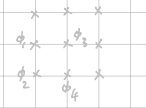
\includegraphics{result.jpg}
\end{center}


We can accelerate this convolution computation using the FFT as normal.

Expressing this more explicitly, when we compute the check potential during the M2L operator during the KIFMM, we compute an approximation of the following integral,


\begin{flalign}
    \phi^c(\mathbf{x}) = \int_{y \in Y} G(\mathbf{x}-\mathbf{y})q(\mathbf{y}) d\mathbf{y}
\end{flalign}

where $\mathbf{x} \in X$ are points on the target surface, $\mathbf{y} \in Y$ are points on the source surface and $q(\mathbf{y})$ are discrete charges placed at source surface points and $\phi^c(\mathbf{x})$ is the check potential at a target surface point. Applying Fourier convolution theorem,

\begin{flalign}
    \phi^c(\mathbf{x}) = \mathcal{F}^{-1} \left[ \mathcal{F} G(\mathbf{\xi}) * \mathcal{F} q(\mathbf{\xi})\right] (\mathbf{x})
\end{flalign}

We notice that $G(\mathbf{\xi})$ must contain all the unique kernel evaluations between points on the source/target surface, and that when convolved with $q(\mathbf{\xi})$ we must recover the potentials in a predictable way (in order to create index maps to the write matrix elements).

This is done by defining a `convolution grid', which is an extension of the surface discretisation of the KIFMM. This extension is defined by the unique evaluations of the Green's function with respect to a single point on the target surface grid. By doing this, the convolution can be drawn around the source surface grid in a formulaic way each time, as represneted by the above figure. Representing the points on the target and surface grids by their indices in their discrete form, i.e. $\mathbf{y} = y_{ijk}$, we can write the matrix elements of the kernel evaluations represented on this convolution grid as,

\begin{flalign}
    \underline{G}_{ijk} = G(x_{000}-y_{ijk})
\end{flalign}

where $x_{000}$ corresponds to the lower left corner of the target surface, though in principle any point on the target surface could be used, they will result in different mappings between the final convolved form and the potentials we're seeking to identify. This results in a 3D sequence,

\begin{flalign}
    G[i, j, k] =  \underline{G}_{ijk} 
\end{flalign}

where the indices, e.g. $i \in I$, extend over the indices of the axes of the convolution grid. 

Next we discuss padding. For optimum performance, the size of the FFT in each dimension should be a power of two. So we begin by padding the convolution grid with zeros,

\begin{equation}
    G^{pad}[i',j',k'] = 
    \begin{cases} 
    0 & 
    \begin{aligned}
            &\text{if } 0 \leq i' \leq P-M \\
            &\text{ and } 0 \leq j' \leq Q-N \\
            &\text{ and } 0 \leq k' \leq R-K \\
    \end{aligned} 
    \end{cases}
\end{equation}

Where $P, Q, R$ correspond to the dimensions of the sequence before padding, and $M, N, K$ correspond to the next largest power of two of the size each of these dimensions, $i', j', k'$ are the indices of the padded array. The remainder of the array is filled by the original sequence $G[i, j, k]$.


Similarly,we must pad the sequence of discrete charges to match the dimensions of the padded kernel sequence in order to compute the FFT. We start by creating a creating a new convolution grid, and placing the discrete charges at their corresponding positions from the source surface grid. Once this is complete, we have a sequence $q[i, j, k]$ with the same dimensions as the kernel sequence. We then choose the following padding,

\begin{equation}
    q^{pad}[i',j',k'] = 
    \begin{cases} 
    0 & 
    \begin{aligned}
            &\text{if } P-M \leq i' \leq P \\
            &\text{ and } Q-N  \leq j' \leq Q \\
            &\text{ and } R-K  \leq k' \leq R \\
    \end{aligned} 
    \end{cases}
\end{equation}

Where $P, Q, R$ are the same as for the kernel sequence, note $M, N, K$ are the same for the kernel and charge sequence now. This choice of padding for both sequences as well as taking the convolution grid with respect to $x_{000}$ is fortuitous. Noting that in the computation of the FFT convolution we must flip the kernel, we find that our sequence of potentials lie at the indices $[P-M-1:P, Q-N-1:Q, R-K-1:R]$ of the final FFT computed result. Looking up the potentials associated with each point on the target surface grid is exactly equivalent to looking up their associated index in the subsequence of the result indexed by $[P-M-1:P, Q-N-1:Q, R-K-1:R]$.

\subsubsection{Accelerating the Hadamard Product}

The Hadamard product is the most computationally intensive part of the above scheme. Here I spell out how to accelerate it using explicit SIMD instructions and careful data organisation which is the approach introduced by \cite{Malhotra2015} and re-implemented in \cite{wang2021exafmm}.

Instead of computing the convolution in the preceding section for a single source and target box, we now consider a set of siblings together,

\begin{flalign}
    S = \cup_{i=1}^{N=8} S_i
\end{flalign}

For a given M2L interaction, we'll have a sequence corresponding to the unique kernel interactions,

\begin{flalign}
    G_l[i, j, k]
\end{flalign}

We generally pre-compute and store the FFTs of these for use, for a given M2L interaction,

\begin{flalign}
    \hat{G}_l[i, j, k]
\end{flalign}

We can organise these in memory in a special way to maximise cache-reuse. Consider a node in a multilevel tree. For each node in its near field's child nodes we can compute $8 \times 8$ unique kernel interactions with respect to the source node's 8 children. This results in a total of $8 \times 8 \times 26 = 1664$ sequences corresponding to FFTs of these. The authors of the \cite{Malhotra2015} proceed by iterating in parallel over each frequency of the resulting Fourier transform, pulling out the corresponding components from these 1664 sequences of Fourier transforms of the kernel function, which results in 26 matrices of size $8 \times 8$ corresponding to the frequency chunk of the convolutions for that neighbour, for each of these matrices we can compute a Hadamard product with an $8 \times 1$ sized vector corresponding to the frequency component for each of the 8 child nodes in our source node. This is an $8 \times 8$ operation that the authors implement using explicit SIMD instructions. The benefit of this scheme is that the Fourier transforms of the kernel, chunked by frequency, are held in memory when applied to the signals, also chunked by frequency, in the source node.


% \begin{algorithm}
%     \caption{M2L Convolution}
%         \begin{algorithmic}[1]
%             \Require level $l$ 
%             \For{Translation Vector $t$}
%                 \parState
                
%                 \State Result for these sibling set, $H$
%                 \For{Siblings FFT sequence, $\hat{S}$, Kernel FFT sequence, $\hat{G}$ }
%                     \State $H[subI, subJ]$ = hadamard\_8x8($\hat{S}_{8x8}$, $\hat{G}_{8x8}$)
%                 \EndFor
%             \EndFor
%     \end{algorithmic}
% \end{algorithm}


\section{A New Software and Algorithm for M2L operators}

We identify a gap in the literature investigating the different approaches to compute the M2L operator. This is likely due to the highly specialised nature of FMM implementations, and the resulting brittleness of the software implementations. With our Rust framework it is easy to plug and play M2L implementations, allowing us to directly compare the performance in terms of accuracy and speed of the two main algorithmic approaches. Here we give an overview of the software's design, it's positioning withing the wider framework for the solution of integral equations. We proceed to describe our favoured implementation approach, which we believe maximally uses the features of modern hardware to increase the throughput (points/sec) of the M2L operation. We benchmark our approach with other FMM softwares.

\subsection{Rusty Field}

By using Rust's traits system we can construct a software contract that specifies a field translation. The difficulty here is designing a contract that is general enough to capture the behaviour of an M2L operation, but also low-level enough to be easily editable and re-implemented. Unfortunately it is not possible to design a contract at the level of a tree node, as many computational optimisation strategies consume the tree's nodes level-by-level.

We use the following interface,


[FIELD INTERFACE CODE]


This allows us to re-implement the M2L for a given method and set of computational optimisations, though we note that it will be difficult for re-implementers or users to design their own high performance implementation without a deep understanding of the software internals.

\subsection{FFT based M2L with Symmetries}

We can extend the scheme introduced by \cite{Malhotra2015} for homogenous and translation invariant kernels using the methods described in \cite{Messner2012} which apply when FMM interpolation points are arranged on a regular grid, as is the case for both the bbFMM and the KIFMM. Instead of computing 1664 convolutions corresponding to  M2L interactions, which contains a lot of redundancy, we can instead compute just 16. This will also result in just 16 Hadamard products instead of 1664. Unlike with the BLAS3/SVD approach, this optimisation will dramatically cut down the FLOP count when using this approach for the convolution, and we therefore believe is the optimum method for computing the M2L operation.

Here we describe the ways to remove redundant M2L translations as described in \cite{Messner2012}. They describe two symmetry planes, axial and diagonal. The axial planes are given by $t_1 = 0$, $t_2 = 0$ and $t_3 = 0$, each dividing $\mathbb{Z}^3$ into two parts, we can combine all three planes to divide $\mathbb{Z}^3$ into octants. We use $\mathbb{Z}^3_+$ as a reference octant. The diagonal planes are given by $t_1 = t_2$, $t_1 = t_3$ and $t_2 = t_3$, in all there are 6 diagonal symettries, however we restrict ourselves to those in the reference octant. By combining the axial and diagonal symmetries we obtain a cone,

\begin{flalign}
    \label{eq:reference_cone}
    \mathbb{Z}^3_{sym} = \left \{ \mathbb{Z}^3_{sym} \subset \mathbb{Z}^3 : t_1 \geq t_2 \geq t_3 \geq 0 \text{ with } t \in \mathbb{Z}^3 \right \}
\end{flalign}

We identify a subset of transfer vectors $T_{sym} = T \cap \mathbb{Z}^3_{sym}$, all other transfer vectors can be expressed as reflections/rotations of this fundamental set. This can be used to construct permutation matrices that can be applied to the M2L operators for these unique transfer vectors, note that this is independent of the way in which these M2L operators are being calculated and therefore applies to either the SVD or FFT approach.

Consider an M2L operator $K_p(t)$, corresponding to one of 316 unique orientations at a given level, any reflection of a transfer vector along a symettry plane determines the permutation of its associated operator as

\begin{flalign}
    K_t = P_t K_{p(t)} P_t^T
\end{flalign}

The permutation matrix $P_t$ depends upon the transfer vector $t \in T$, where we also need a surjective mapping $p : T \rightarrow T_{sym}$ that associates each transfer vector in $T$ with exactly one in $T_{sym}$. The left application corresponds to a permutation of the rows, and the right the columns of the original matrix. The permutation matrices depend only upon the transfer vector $t$ and are constructed as follows.


\begin{list}{-}{Discussion}
    \item Why is this better than the SVD approach (complexity analysis)
    \item Why it doesn't make sense to necessarily take advantage of symettries with SVD approach - flop count same, experiments to prove that BLAS3 doesn't make much difference.
    \item Outline of algorithm.
\end{list}

\subsection{Investigations}

\begin{list}{-}{Benchmark figures}
    \item Accuracy of svd method as a function of p and k, accuracy of fft method as a function of p.
    \item FLOP counts of both methods vs accuracy, ie. complexity analysis.
    \item Absolute speeds of both methods.
\end{list}

\section{Appendix}

\subsection{Fourier Transform Theoretical Background}

A lot of the theoretical background I want to keep at hand is taken from the excellent course notes \cite{Osgood2014}. I summarise the key aspects here as related to the FFT, especially when discussing padding/indexing, as these issues come up most pertinently in real implementations.

\subsubsection{Going from Fourier Series to Fourier Transforms}

Starting off with Fourier Series (FS), i.e. representing periodic functions using a periodic (trig) basis, and generalising to non-periodic (i.e. $\infty$ period) functions takes us to Fourier Transforms (FT).

Q: Is the sum of two periodic functions also periodic? 

A: No if you're a mathematician, e.g. $cos(t)$ and $cos(\sqrt{2}t)$ are each periodic with periods $2\pi$ and $2\pi/\sqrt{2}$ resp. But the sum is not periodic. ie. no common divisors in the periods.

When considering a sum of sinusoids, as Fourier pitched, 

\begin{flalign}
    \sum_{n=1}^N A_n \sin(n \theta + \phi_n)
\end{flalign}

The sum is also periodic as the frequencies are multiples of the fundamental frequency $1/2\pi$.

It's more common to write a general trig sum as,

\begin{flalign}
    \frac{a_0}{2} + \sum_{n=1}^N (a_n \cos(2\pi nt) + b_n \sin(2\pi nt))
\end{flalign}

Where the zeroth component is often referred to as a DC component (from electrical engineering contexts). The half is a simplifying factor that comes up. Expressing this instead using complex exponentials, the sum can be written as,

\begin{flalign}
    \sum_{n=-N}^N c_n e^{2\pi i nt}
\end{flalign}

One can refer to RHB to see how the coefficients are related between forms. In particular we find $c_0 = a_0 / 2$. The complex conjugate property of the coefficients,

\begin{flalign}
    c{-n} = \bar{c_n}
\end{flalign}

is important, it allows us to group terms such that

\begin{flalign}
    \sum_{n=-N}^N c_n e^{2\pi i nt} = 2 \text {Re} 
    \left \{ \sum_{n=0}^N c_n e^{ 2 \pi i n t} \right \}
\end{flalign}


Our goal is to express a general periodic function $f(t)$ as an FS.

\begin{flalign}
    f(t) = \sum_{-N}^N c_n e^{2\pi i n t}
\end{flalign}

Take a given coefficient, can we solve for it ? 

\begin{flalign}
    f(t) &= \sum_{-N}^N c_n e^{2\pi i n t} \\
    e^{-2 \pi i k t} f(t)  &= e^{-2\pi i k t} \sum_{-N}^N c_n e^{2\pi i n t}
\end{flalign}

Therefore,

\begin{flalign}
    c_k =  e^{-2 \pi i k t} f(t) - \sum_{n=-N, n \neq k}^N c_n e^{2\pi i (n-k) t}
\end{flalign}

We've pulled the coefficient out, but the expression involves all the other coefficients! Instead, we can try and integrate both sides over 0 to 1 (any function can be made to have this period if it's periodic). The integrals in the sum all cancel out,

\begin{flalign}
    \int_0^1 e^{2\pi (n-k)t}dt = \frac{1}{2\pi i (n-k)} e^{2\pi i (n-k)t} |_{t=0}^{t=1} = 0
\end{flalign}

With this trick, the expression for the coefficient reduces to,

\begin{flalign}
    c_k = \int_{0}^1  e^{-2 \pi i k t} f(t) dt
\end{flalign}

We haven't stated whether any periodic function \textit{can} be expressed in such a way that we can apply this analysis, but if we can express it in the periodic form we started off with, we have a way of evaluating the coefficients.

Note in particular that the zeroth coefficients corresponds to an average value of the function over its period.

\begin{flalign}
    \hat{f}(0) = \int_{0}^{1} f(t) dt
\end{flalign}

The case when all the coefficients are real is when the signal is real and even. For then,

\begin{flalign}
    \bar{\hat{f}}(n) &= \hat{f}(-n) = \int_{0}^{1} e^{-2\pi i (-n) t} f(t) dt = \int_{0}^{1} e^{2\pi i n t}f(t) dt \\ 
    &= -\int_{0}^{-1} e^{-2\pi i n s} f(-s) ds, \text{  subs t = -s, changing lims} \\
    &= \int{-1}^0  e^{-2\pi i n s} f(-s) ds, \text{ even f(s)} \\
    &= \hat{f}(n)
\end{flalign}

So the coefficients are real. The evenness of $f$ seems to pass over into its fourier coefficients too.

We haven't yet answered when a periodic function can be approximated by a fourier series \dots We're basically allowed to if $f(t) \in L^2([0, 1])$ as then the integral defining its Fourier coefficients exists. The fourier approximation is the best approximation in $L^2([0, 1])$ by a trigonemtric polynomial of degree $N$. The complex exponentials form a basis for this space, and the partial sums converge to $f(t)$ in its norm,

\begin{flalign}
    \lim_{N \rightarrow \infty} \left \| \sum_{n=-N}^{N} \hat{f}(n) e^{-2\pi i n t} - f(t) \right \| = 0
\end{flalign}

For Fourier Transforms, lets start off by considering a box function.

\begin{flalign}
    \Pi(t) = \begin{cases}
        1 & \text{if } |t| < 1/2, \\
        0 & \text{if } |t| \geq 1/2.
    \end{cases}
\end{flalign}

This isn't periodic, and doesn't have an FS. However, if we make it repeat with intervals $T$, we can find a representation with coefficients given by,

\begin{flalign}
    c_n = \frac{1}{T} \int_{0}^T e^{-2 \pi i n t / T}f(t) dt =  \frac{1}{T} \int_{-T/2}^{T/2} e^{-2 \pi i n t / T}f(t) dt = \frac{1}{\pi n } \sin(\frac{\pi n }{T})
\end{flalign}

The coefficients tend to 0 for large $T$ as $1/T$, to compensate for this we can scale by $T$. Using a change of variables $s = n/T$ we can write,

$\Pi (s) = \frac{\sin(\pi s)}{\pi s}$

We can now take a limit as $T \rightarrow \infty$,

\begin{flalign}
    \hat{\Pi}(s) = \int_{-\infty}^{\infty} e^{-2\pi i s t} \Pi (t) dt = \int_{-1/2}^{1/2} e^{-2\pi i s t} \cdot 1 dt =  \frac{\sin(\pi s)}{\pi s}
\end{flalign}

We are lead to the same idea - scale the Fourier coefficients by $T$ - if we had started off periodising any function that is zero outside of some interval and letting the period tend to infinity. This gives us the following definition for Fourier Transforms,

\begin{flalign}
    \hat{f}(s) = \int_{-\infty}^{\infty} e^{-2 \pi i s t} f(t) dt
\end{flalign}

where the coefficients are in general complex. FTs produce continuous spectra, in contrast to a discrete set of (potentially infinitely many) frequencies as in FS.

We can push this to get a definition for the dual, the inverse transform. Again supposing that we have a non-periodic function that we can say is zero outside of an interval, we find an expression for its FS, and fourier coefficients

\begin{flalign}
    f(t) = \sum_{n=-\infty}^{\infty} c_n e^{2\pi i n t/T}    
\end{flalign}

\begin{flalign}
    c_n &= \frac{1}{T} \int_{-T/2}^{T/2} e^{-2 \pi i n t / T}f(t) dt = \frac{1}{T}  \int_{-\infty}^{\infty} e^{-2 \pi i n t / T}f(t) dt \\
    & \text{ extension to infty ok as zero outside interval} \\
    &= \frac{1}{T}\hat{f}(\frac{n}{T}) = \frac{1}{T}\hat{f}(s)
\end{flalign}

Plugging back in, and thinking of Riemann sum to approximate an integral,

\begin{flalign}
    f(t) = \sum_{-\infty}^{\infty} \frac{1}{T} \hat{f}(s_n) e^{2 \pi i s_n t} = \sum_{-\infty}^{\infty} \hat{f}(s_n) e^{2 \pi i s_n t} \Delta s \approx \int_{-\infty}^{\infty}\hat{f}(s_n) e^{2 \pi i s_n t} ds
\end{flalign}
\subsubsection{The Convolution}

In general we want to modify signals by each other. Is there a combination of signals $f(t)$ and $g(t)$ such that in the frequency domain the FT is:

$$
\mathcal{F} g(s) \mathcal{F} f(s)
$$

i.e. is there a combination of the signals such that frequency components are scaled by each other?

Very roughly, we find,

\begin{flalign}
    \mathcal{F} g(s) \mathcal{F} f(s) &= \int_{-\infty}^{\infty} e^{- 2 \pi i s t} g(t) ds \int_{-\infty}^{\infty} e^{- 2 \pi i s x} f(x) dx \\
    &=   \int_{-\infty}^{\infty}  \int_{-\infty}^{\infty}  e^{- 2 \pi i s (t+x)} g(t) f(x) dt dx
\end{flalign}

using the change of variable $u = t+x$ for the inner integral,

\begin{flalign}
    \int_{-\infty}^{\infty} \left ( \int_{-\infty}^{\infty} e^{-2 \pi i s u} g(u-x) du \right ) f(x) dx
\end{flalign}

switching the order of integration,

\begin{flalign}
    \int_{-\infty}^{\infty} e^{-2 \pi i s u} \left ( \int_{-\infty}^{\infty}  g(u-x)  f(x) dx \right )du
\end{flalign}

The inner integral can be seen to be a function of $u$, we can write it as $h(u)$, the outer integral reduces to:

\begin{flalign}
    \int_{-\infty}^{\infty}  e^{-2 \pi i s u} h(u) du = \mathcal{F}h (s)
\end{flalign}

This defines our convolution,

\begin{flalign}
    (g * f)(t) =  h(t) = \int_{-\infty}^{\infty} g(t-x) f(x) dx
\end{flalign}

And the following theorem,

\begin{flalign}
    \mathcal{F} (g * f) (s) = \mathcal{F} g(s) \mathcal{F} f(s)
\end{flalign}

Most significantly for us, convolving in the time domain reduces to a multiliplication in the frequency domain.

The convolution is defined by flipping the kernel, and dragging it over the signal.

\subsubsection{Discrete Fourier Transforms, and the Fast Fourier Transform}

We want to find a discrete analogue to the FT for real signals which are sampled at a certain rate.

Let's suppose that $f(t)$ is zero outside of an interval $0 \leq t 
\leq L$, similarly the FT $\mathcal{F} f(s)$ is assumed zero outside of $0 \leq s \leq 2B$ (indexing is easier if we ignore negative frequencies), $L$ and $B$ are both integers.

According to Shannon, we can reconstruct $f(t)$ perfectly if we sample at a rate of $2B$ per second. So in total we want,

$$
N = \frac{L}{1/2B} = 2BL
$$

evenly spaced samples, notice that this is even. Sampled at points,

$$
t_0 = 0, t_1 = \frac{1}{2B},..., t_{N-1} = \frac{N-1}{2B}
$$


\begin{flalign}
    f_{discrete}(t) = \sum_{n=0}^{N-1}\delta (t-t_n)f(t_n)
\end{flalign}

and therefore,

\begin{flalign}
    \mathcal{F}f_{discrete}(t) =  \sum_{n=0}^{N-1} f(t_n) \mathcal{F} \delta (t-t_n) =  \sum_{n=0}^{N-1} f(t_n)  e^{-2\pi i s t_n}
\end{flalign}

which is almost what we need, it's the continuous FT of the sampled form of $f(t)$.

Shifting to the frequency domain, we find the number of sample points to be,

$$
N = \frac{2B}{1/L} = 2BL
$$

the same as in the time domain. We base the discrete version of the FT using the discrete version of the signal,

\begin{flalign}
    F(s_0) = \sum_{n=0}^{N-1}f(t_n)e^{-2 \pi i s_0 t_n}
\end{flalign}

etc. We now have a way of converting from the discrete signal to the discrete FT,

\begin{flalign}
    F(s_m) = \sum_{n=0}^{N-1} f(t_n) e^{-2 \pi i s_m t_n}
\end{flalign}

It's possible to link this to the continuous case by discretising the integral defining a continuous FT, we see that this sum (up to a scaling) comes out.

using,

\begin{flalign}
    t_n = \frac{n}{2B}, \> \> s_m = \frac{m}{L}
\end{flalign}

we can write in terms of indices,

\begin{flalign}
    F(s_m) = \sum_{n=0}^{N-1} f(t_n) e ^{-2\pi i n m / 2BL} = \sum_{n=0}^{N-1} f(t_n) e ^{-2\pi i n m / N } 
\end{flalign}

Thinking about io as sequences of numbers, we can write in `array' form, where the transform is just defined on a sequence.

\begin{flalign}
    \mathbf{F}[m] = \sum_{n=0}^{N-1} \mathbf{f}[n] e^{-2\pi i m n /N}, \> \> m=0, 1, ..., N-1
\end{flalign}

The input sequence can be complex, it's not less valid, but the output sequence is always complex.

A common notation is to write the complex exponentials as,

$$
\omega = e ^{2 \pi i /N} = \omega_N
$$

s.t.

$$
\omega_N^N = 1
$$

for any integer $n$ and $k$,

$$
\omega^{Nn}_N = 1
$$

$$
\omega^{Nn+k}_N = \omega_N^k
$$

and,

$$
\omega_N^{N/2} = -1
$$

so,

$$
\omega_N^{kN/2} = (-1)^k
$$

We write a vector of the $N$th roots of unity as,

$$
\mathbf{\omega} = (1, \omega, \omega^2, ..., \omega^{N-1})
$$

the components,

$$
\mathbf{\omega}^k[m] = \omega^{km}
$$

The DFT can be thought of as a linear transfrom between $\mathbb{C}^N$ to $\mathbb{C}^N$. This linear transform can be explicitly written out as a matrix, which I won't bother with here, look at 257 in \cite{Osgood2014}.

This is a dense $N \times N$ matrix! The FT is in general hard to compute, hence the revolution of the FFT which can do it in log-linear time.


\subsection{$N$-Dimensional DFT}

The DFT takes a sequence of complex numbers $u_0, u_1, ..., u_{N-1}$ and transforms them into another sequence of complex numbers $\hat{u}_0, \hat{u}_1,...,0\hat{u}_{N-1}$, the forward and backwatf transfroms is defined as,

\begin{flalign}
    \hat{u}_k = \frac{1}{N}\sum_{j=0}^{N-1}u_j e^{-ikx_j}, \> \> k=0,1,...,N-1 \\
    u_k = \frac{1}{N}\sum_{j=0}^{N-1}\hat{u}_j e^{ikx_j}, \> \> k=0,1,...,N-1
\end{flalign}

where $x_j = 2\pi j / N$. If instead the data is arranged in a multidimensional array, $u_{j_0, j_1, ..., j_{d-1}}$ where there are $d$ index sets $j_m = 0, 1, ..., N_{m-1}$, $m \in 0, 1, ..., d-1$ with $N_m = \|j_m\|$ being the length of $j_m$. A forward $d$-dimensional DFT of the $d$-dimensional array will be computed as,

\begin{flalign}
    \hat{u}_{k_0, k_1, ..., k_{d-1}} = \sum_{j_0 = 0}^{N_0 - 1} 
    \left( \frac{\omega_0^{k_0 j_0}}{N_0} \sum_{j_1 = 0}^{N_1-1} \left(  \frac{\omega_1^{k_1j_1}}{N_1} ... \sum_{j_d-1}^{N_{d-1}-1} \frac{\omega_{d-1}^{k_{d-1}j_{d-1}}}{N_{d-1}} u_{j_0, j_1,...,j_{d-1}} \right) \right)
\end{flalign}

where $w_j = e^{\frac{-2\pi i}{N_j}}$


Normalisation in this context refers to the scaling of the output to be independent of input size. That is if you double the size of your input, e.g. via padding, the amplitude of the output frequencies should not change. This is done by dividing the output of the FFT by the length of the input array (or its square root depending on convention).

\subsection{Method of Fundamental Solutions (MFS)}\label{app:mfs}

We can use MFS to approximate the field due to a set of discrete charges, by using the fundamental solutions as a basis, this is the approach taken by the authors of the KIFMM \cite{Ying2004}. This note is based on exposition presented in \cite{barnett2008stability}, and adapted to the field approximations required in the KIFMM - our problem of interest.

Our goal during the FMM is to approximate either (a) the potential generated by particles inside a tree node in the exterior, (b) the evaluate the approximation of the potential generated by particles outside of a tree node inside its interior. The KIFMM achieves this using the method of fundamental solutions (MFS). Consider problem (a), sketched in figure \ref{app:fig:upward_surface}. The MFS approximation is to approximate the potential by using a linear cobination of fundamental solutions of the problem at hand,

\begin{flalign}
    u(\mathbf{x}) \approx u^N(\mathbf{x}) = \sum_{i \in I_u^B} G(\mathbf{x}, \mathbf{y}_i)\phi_i
\end{flalign}

Here we use $N$ points on an `equivalent' surface, that encloses the node containing the points, specified by the index set of the points $I_u^B$ the reason for denoting this with $u$ in particular will become apparent later, $\phi_i$ are some unknown densities representing the charges contained in the node which we are to solve for and $G(., .)$ denotes the Green's function. In order to do this, we can calculate directly the potential generated by points contained in the node at the (blue) check surface,

\begin{flalign}
    \sum_{i \in I_s^B} G(\mathbf{x}, \mathbf{y}_i)\phi_i = q^{B, u}
\end{flalign}

which we call the check potential. The potential due to our charges is guaranteed to be equivalent to that generated by our equivalent charges due to the uniqueness of the exterior problem for our kernels of interest (e.g. Laplace). 

We see that our MFS approximation is analogous to an approximation of a single-layer potential defined along the equivalent surface, $\Gamma_e$, with some continuous density $\phi$

\begin{flalign}\label{app:eq:mfs}
    u(\mathbf{x}) \approx \int_{\Gamma_e} G(\mathbf{x}, \mathbf{y})\phi(\mathbf{y}) d\mathbf{y}
\end{flalign}

if we replace $\phi(\mathbf{y})$ with $\sum_{j=1}^{N}\phi_i \delta(\mathbf{y}-\mathbf{y}_j)$. Therefore the MFS approximates a first-kind integral equation, which is in general ill-conditioned [TODO - lookup in Kress].

We can solve this ill-conditioned system using Tikhonov regularisation to convert this first kind integral equation into a second-kind integral equation. Written in matrix form our problem becomes

\begin{flalign}
    K \phi = q
\end{flalign}

Where $K$ is the discretisation of the matrix elements described by equation (\ref{app:eq:mfs}), $\phi$ is a vector containing the densities supported on the equivalent surface, and $q$ is a vector of check potentials evaluated on the check surface. Applying Tikhonov regularisation,

\begin{flalign}
    \phi = (\alpha I + K^* K)^{-1} q
\end{flalign}

we can solve for $q$, where we choose the regularisation parameter experimentally. 

The procedure described above amounts to the P2M operator in the FMM, the other FMM operators in the KIFMM are calculated in in a highly similar manner and we won't bother describing them here. The key thing to note here is that this approximation method relies only on evaluating the fundamental solutions (kernels) of the PDE, we don't need to actually write out an analytic expansion to approximate the potential in the exterior, instead we just need to find a set of equivalent densities and we can reconstruct the exterior field using the MFS. The literature shows that one can achieve exponential convergence with increasing $N$ \cite{barnett2008stability}.

\begin{figure}\label{app:fig:upward_surface}
\centering
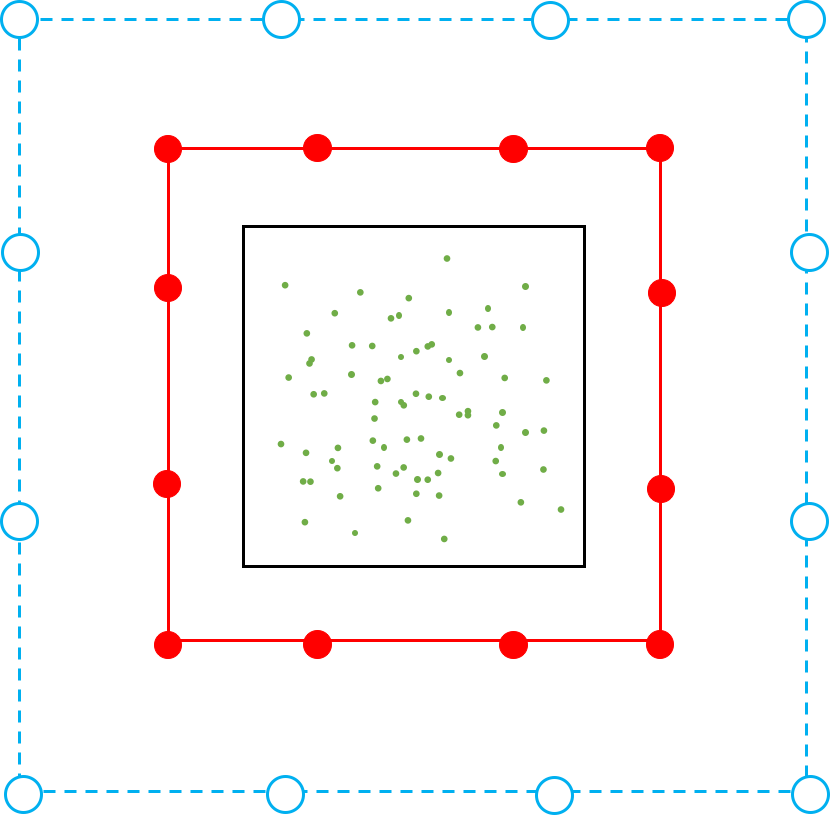
\includegraphics[width=5cm]{upward_surface.png}
\caption{A set of particles contained in a tree node (green), enclosed by the tree node (black), an equivalent surface (red) and a check surface (blue check).}
\end{figure}
    
\printbibliography[heading=bibintoc]

\end{document}
